\input{../../input/main}

\begin{document}

\begin{center}
  \Large{\textbf{Городской центр физического образования, 10 класс.}\\
  \textit{Серия 15, 29 января 2015.}}
\end{center}

\begin{center}
  \large\textbf{ Ещё немного термодинамики. }
\end{center}

%\large

\task{ В герметичном кубе объёма $V$ находится аргон. При низкой
  температуре сила давления на все стенки, кроме нижней, равна 0, а
  сила давления на нижнюю равна $F_0$. Найдите силу, действующую на
  верхнюю стенку при комнатной температуре $T$, считая, что весь аргон
  находится в газообразном состоянии. Ускорение свободного падения
  $g$. Молярная масса аргона $\mu$. В данной задаче при комнатной
  температуре аргон можно считать идеальным газом. }

\taskpic{ На рисунке изображена зависимость объема идеального газа от
  температуры. В какую сторону изменялось давление газа на различных
  участках кривой в процессе перехода из состояния 1 в состояние 2? }
{
  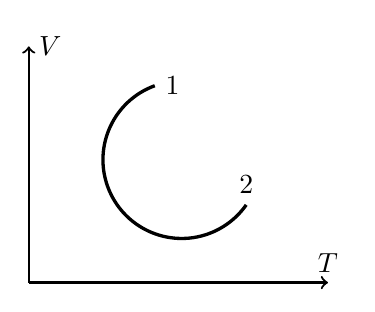
\begin{tikzpicture}
    \draw[thick,->] (0,0) -- (3.8,0) node[above] {$T$};
    \draw[thick,->] (0,0) -- (0,3) node[right] {$V$};
    \draw[very thick] (1.6,2.5) node[right] {1} arc (110:325:1cm)
    node[above] {2};
  \end{tikzpicture}
}

\task{ Идеальный газ участвует в процессе, в ходе которого его
  давление, объем и температура меняются. Зависимость от времени
  давления и объема газа представлена на графиках. Постройте график
  зависимости от времени для температуры газа. В начальный момент
  температура газа была равна $T_0$, величина $t_0$ известна. }

\begin{figure}[h]
  \centering
  \subcaptionbox{}
  {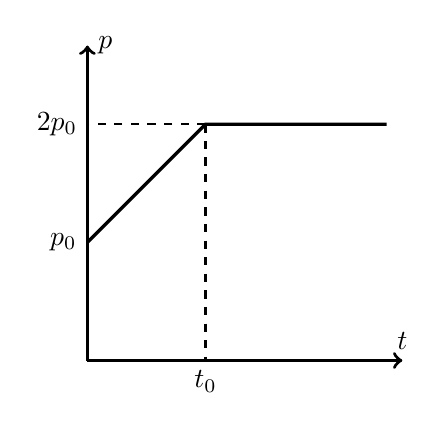
\begin{tikzpicture}
      \draw[very thick, ->] (0,0) -- (4,0) node[above] {$t$};
      \draw[very thick, ->] (0,0) -- (0,4) node[right] {$p$};
      \draw[very thick] (0,1.5) node[left] {$p_0$} -- (1.5,3) --
      (3.8,3); 
      \draw[thick,dashed] (1.5,3) -- (1.5,0) node[below] {$t_0$};
      \draw[thick,dashed] (1.5,3) -- (0,3) node[left] {$2p_0$};  
    \end{tikzpicture}}
    \qquad
    \subcaptionbox{}
    {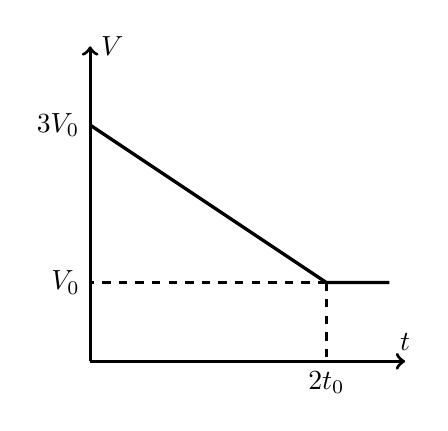
\begin{tikzpicture}
      \draw[very thick, ->] (0,0) -- (4,0) node[above] {$t$};
      \draw[very thick, ->] (0,0) -- (0,4) node[right] {$V$};
      \draw[very thick] (0,3) node[left] {$3V_0$} -- (3,1) --
      (3.8,1); 
      \draw[thick,dashed] (3,1) -- (3,0) node[below] {$2t_0$};
      \draw[thick,dashed] (3,1) -- (0,1) node[left] {$V_0$};  
    \end{tikzpicture}}
\end{figure}

\task{ В цилиндре под поршнем площади $S$ находится 1 моль
  газа. Поршень прикреплен к дну цилиндра пружиной. Изначально его
  удерживают так, что пружина не растянута, при этом объем газа
  $V_{0}$, а давление $P_{0}$. Над газом производят циклический
  процесс. Сначала газ расширяется изотермически, получая при этом
  тепло $Q$. Затем цилиндр теплоизолируют и уменьшают внешнюю силу
  давления на поршень, пока она не станет нулевой. После этого газ
  изотермически сжимают до изначального объема и изохорически
  переводят в исходное состояние. Определите, при какой жесткости
  пружины работа такой тепловой машины, совершаемая за цикл, будет
  нулевой. \textit{Примечание 1}: работа $A$ 1 моля газа при
  изотермическом расширении от объема $V_0$ до $V$
  $A = R T \mathrm{ln} \left(V/V_0 \right)$. \textit{Примечание 2}:
  Основное свойство логарифма: $e^{\mathrm{ln}x}=x$. }

\end{document}


%%% Local Variables: 
%%% mode: latex
%%% TeX-engine:xetex
%%% TeX-PDF-mode: t
%%% End:
